\documentclass[a4paper]{article}
\usepackage[T1,T2A]{fontenc}
\usepackage[utf8]{inputenc}
\usepackage[english,russian]{babel}
\usepackage{booktabs}
\usepackage{color,colortbl}
%\usepackage{amsmath}
%\usepackage{amsfonts}
%\usepackage{amssymb}
%\usepackage{makeidx}
\usepackage{listings}
\usepackage{graphicx}
\definecolor{green}{RGB}{45,140,31}
\definecolor{darkishgreen}{RGB}{39,203,22}
\definecolor{LightCyan}{rgb}{0.88,1,1}
\definecolor{Gray}{gray}{0.9}
\definecolor{lightRed}{RGB}{230,170,150}
\definecolor{modRed}{RGB}{230,82,90}
\definecolor{strongRed}{RGB}{230,6,6}

\lstset{ %
  language=SQL,                % Язык программирования
  numbers=left,                   % С какой стороны нумеровать
  extendedchars=\true,
  %numberstyle=tinycolor{gray},     % Стиль который будет использоваться для нумерации строк
  %stepnumber=2,                   % Шаг между линиями. Если 1, то будет пронумерована каждая строка
 % numbersep=5pt,
 % backgroundcolor=color{white},      % Цвет подложки. Вы должны добавить пакет color - usepackage{color}
  showspaces=false,
  showstringspaces=false,
  showtabs=false,
  %frame=single,                    % Добавить рамку
  %rulecolor=color{black},
  tabsize=4,                       % Tab - 2 пробела
  breaklines=true,                 % Автоматический перенос строк
  breakatwhitespace=true,          % Переносить строки по словам
  title=lstname,                   % Показать название подгружаемого файла
  keywordstyle=\color{green},          % Стиль ключевых слов
  %commentstyle=color{dkgreen},       % Стиль комментариев
  %stringstyle=color{mauve}          % Стиль литералов
}

\usepackage[english,russian]{babel}

\begin{document}

\section{Лабораторная работа. Основы работы с базами данных}

Цель работы:

\subsection{Теоретические основы}

Хранение информации – одна из важнейших функций компьютера. Одним из распространенных средств такого хранения являются базы данных.\linebreak
\textbf{База данных (БД)} --- совокупность взаимосвязанных, хранящихся вместе данных при наличии такой минимальной избыточности, которая допускает их использование оптимальным образом для одного или нескольких приложений. Создание базы данных, ее поддержка и обеспечение доступа пользователей к ней осуществляется централизованно с помощью специального программного инструментария --- системы управления базами данных.\linebreak
\textbf{Система управления базами данных (СУБД)} --- это комплекс программных и языковых средств, необходимых для создания баз данных, поддержания их в актуальном состоянии и организации поиска в них необходимой информации. Концептуальная модель БД описывает сущности, их свойства и связи между ним и не зависит от конкретной СУБД.\linebreak
\textbf{Сущность} --- это реальный или представляемый тип объекта, информация о котором должна сохраняться и быть доступна. В диаграммах сущность представляется в виде прямоугольника, содержащего имя сущности. При этом имя сущности – это имя типа, а не некоторого конкретного экземпляра этого типа. Примеры сущностей: КАФЕДРА, ГРУППА, СТУДЕНТ. Каждый экземпляр сущности (объект) должен быть отличим от любого другого экземпляра той же сущности. Пример экземпляров сущности КАФЕДРА: КиПР, ЭГН, ТММСиИ, сущности СТУДЕНТ: Иванов А.П., Петрова Н.Н. \linebreak
\textbf{Связь} --- это ассоциация, устанавливаемая между двумя сущностями. Связь может существовать между двумя разными сущностями или между сущностью и ей же самой (рекурсивная связь). Возможны связи на основе отношений:
\begin{itemize}
    \item один-к-одному
    \item один-ко-многим
    \item многие-ко-многим
\end{itemize}

Связь «Один-ко-многим»: ГРУППА содержит много СТУДЕНТОВ. Каждый СТУДЕНТ входит только в одну ГРУППУ. Связь «Многие-ко-многим»: СОБАКА может укусить много ЧЕЛОВЕК, ЧЕЛОВЕК может быть укушен многими СОБАКАМИ. Связь "один к одному" встречается редко. Например, у нас есть таблица с информацией о всех сотрудниках и таблица с информацией о всех торговых агентах, которые являются сотрудниками нашего предприятия. Записи в таких таблицах могут быть связаны отношением "один к одному".

\subsubsection{Свойства сущностей}
Сущности имеют свойства, которые называются атрибутами.
Например, атрибуты:

сущности КАФЕДРА:
    \begin{itemize}
      \item название
      \item год создания
    \end{itemize}

сущности ГРУППА:
\begin{itemize}
    \item номер
    \item специальность
\end{itemize}

сущности СТУДЕНТ:
\begin{itemize}
\item фамилия
\item имя
\item отчество
\item номер студенческого билета
\item номер паспорта
\item год рождения
\item месяц рождения
\item день рождения
\end{itemize}

Любой атрибут принимает значения из некоторого множества допустимых значений, называемого доменом атрибута.

Например:
\begin{itemize}
    \item домен атрибута «год создания»: целые положительные числа;
    \item домен атрибута «имя»: строка, не содержащая пробелов;
    \item домен атрибута «год рождения»: целые положительные числа;
    \item домен атрибута «месяц рождения»: январь, февраль, март … декабрь;
    \item домен атрибута «день рождения»: целые числа от 1 до 31.
\end{itemize}

\subsubsection{Ключ сущности}

\textbf{Ключ сущности (entity key), первичный ключ} --- это атрибут (или множество атрибутов) уникальным образом идентифицирующих экземпляр сущности (объект). Например: ключ сущности СТУДЕНТ – номер студенческого билета, ключ ФАКУЛЬТЕТА --- название. Если ключ состоит из одного атрибута, его называют простым ключом. Если ключ сущности состоит из нескольких атрибутов, его называют составным ключом. Например, для сущности ДОМ с атрибутами «улица», «этажность», «год постройки», «номер дома», первичным ключом будет «улица»+ «номер дома».

\subsubsection{Реляционная модель данных}

Понятие реляционный (англ. relation --- отношение) связано с разработками известного американского специалиста в области систем баз данных Е.Кодда. Реляционная модель ориентирована на организацию данных в виде двумерных таблиц. Каждая реляционная таблица представляет собой двумерный массив и обладает следующими свойствами:

\begin{itemize}
    \item каждый элемент таблицы --- один элемент данных
    \item все столбцы в таблице однородные, т.е. все элементы в столбце имеют одинаковый тип (числовой, символьный и т.д.) и длину
    \item каждый столбец имеет уникальное имя (заголовки столбцов являются названиями полей в записях)
    \item одинаковые строки в таблице отсутствуют
  \item порядок следования строк и столбцов может быть произвольным
\end{itemize}

\textbf{Отношение} --- это плоская таблица, содержащая N столбцов, среди которых нет одинаковых. \textbf{N} --- это степень отношения, или арность отношения. Столбец отношения соответствует атрибуту сущности. \textbf{Кортеж} --- строка отношения (соответствует записи в таблице).

\textbf{Пример реляционной модели}

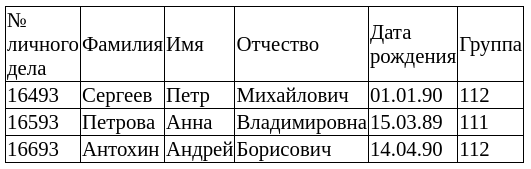
\includegraphics[width=\textwidth]{db1.png}

Отношения представлены в виде таблиц, строки которых соответствуют кортежам или записям, а столбцы --- атрибутам отношений, доменам, полям. Поле, каждое значение которого однозначно определяет соответствующую запись, называется простым ключом (ключевым полем). Если записи однозначно определяются значениями нескольких полей, то такая таблица базы данных имеет составной ключ. В примере ключевым полем таблицы является "№ личного дела".

\subsection{Практическая часть}

LibreOffice Base позволяет создавать как локальные, так и сетевые реляционные базы данных или подключаться к уже имеющимся базам. В любом случае Base позволяет добавлять и удалять записи, редактировать данные, делать выборки, формировать отчеты.

\subsubsection{Создание базы данных}
При запуске LibreOffice Base предлагает создать новый файл базы данных или выбрать уже созданный, или подключится к существующей базе данных.

Для создания новой базы данных нужно выбрать первый пункт. Затем нажать Далее и выбрать Зарегистрировать базу данных и Открыть базу для редактирования. При завершении работы мастера потребуется указать имя новой базы и место для сохранения файла с ней. После этого открывается окно для работы с базой.

\begin{figure}[h]
\center{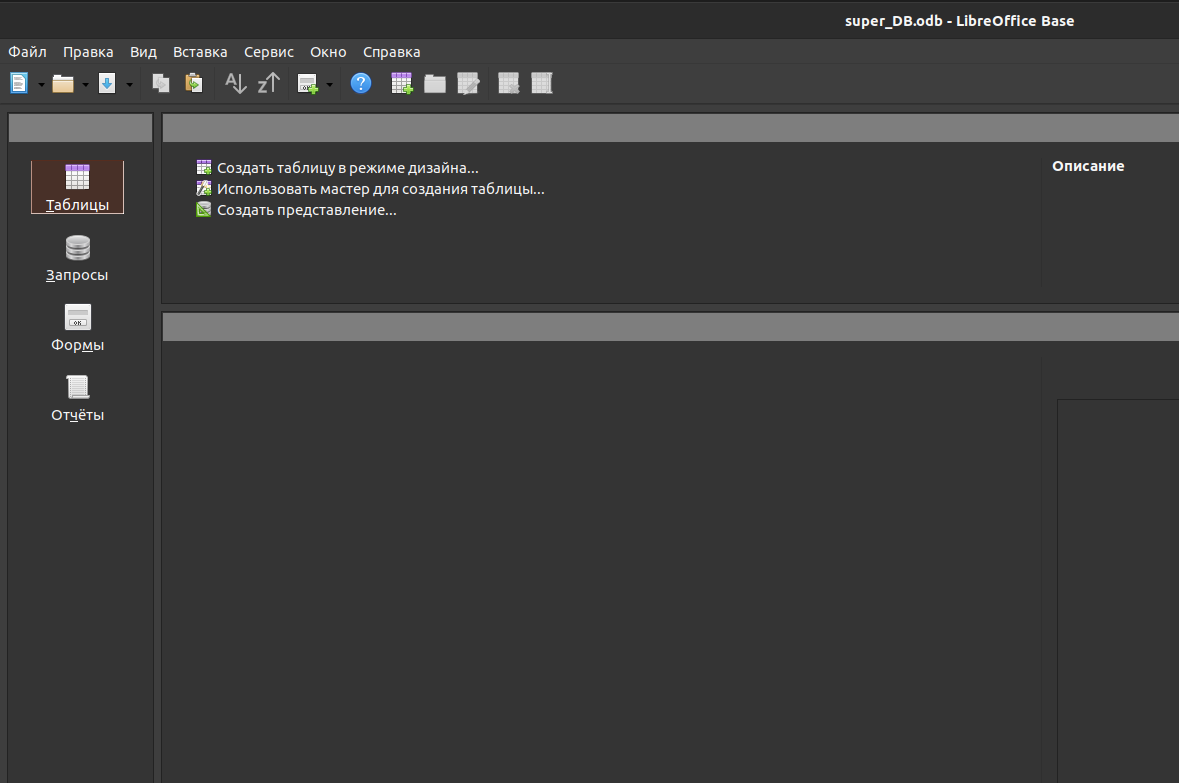
\includegraphics[width=\textwidth]{db2_main.png}
  \caption{Главное меню}\label{ris:main}}
\end{figure}

\subsubsection{Создание таблиц}

Во вкладке таблицы предоставляется выбор создания таблиц в дизайнере или по существующему шаблону с помощью мастера. Мы будем пользоватся дизайнером таблиц. При щелчке левой кнопкой мыши на элементе Таблицы, в правой нижней части рабочего поля будут перечислены имеющиеся таблицы, сейчас там пусто. В правой верхней части рабочего поля появляется набор возможных действий. Удобнее всего создавать таблицы в режиме дизайна. Для этого надо выбрать верхний пункт, после чего откроется соответствующее окно. Каждая строка окна Дизайнера таблиц (Table Disign) описывает одну колонку создаваемой таблицы. Первая строка Дизайнера соответствует первой колонке таблицы, вторая строка - второй колонке и так далее. На иллюстрации строки Дизайнера уже заполнены для создания конкретной таблицы. Проектирование таблицы --- ответственный этап создания базы данных. Ошибки, допущенные при проектировании таблицы потом сложно или вообще невозможно исправить.

При проектировании таблицы нужно обратить внимание на два основных момента. Перечень и порядок следования колонок определяют те данные об объекте, которые будут заноситься в базу и то, насколько удобно это будет делать. А свойства этих данных определяют размер файла базы. Это можно пояснить на примере показанной здесь таблицы студенты.

\begin{figure}[h]
\center{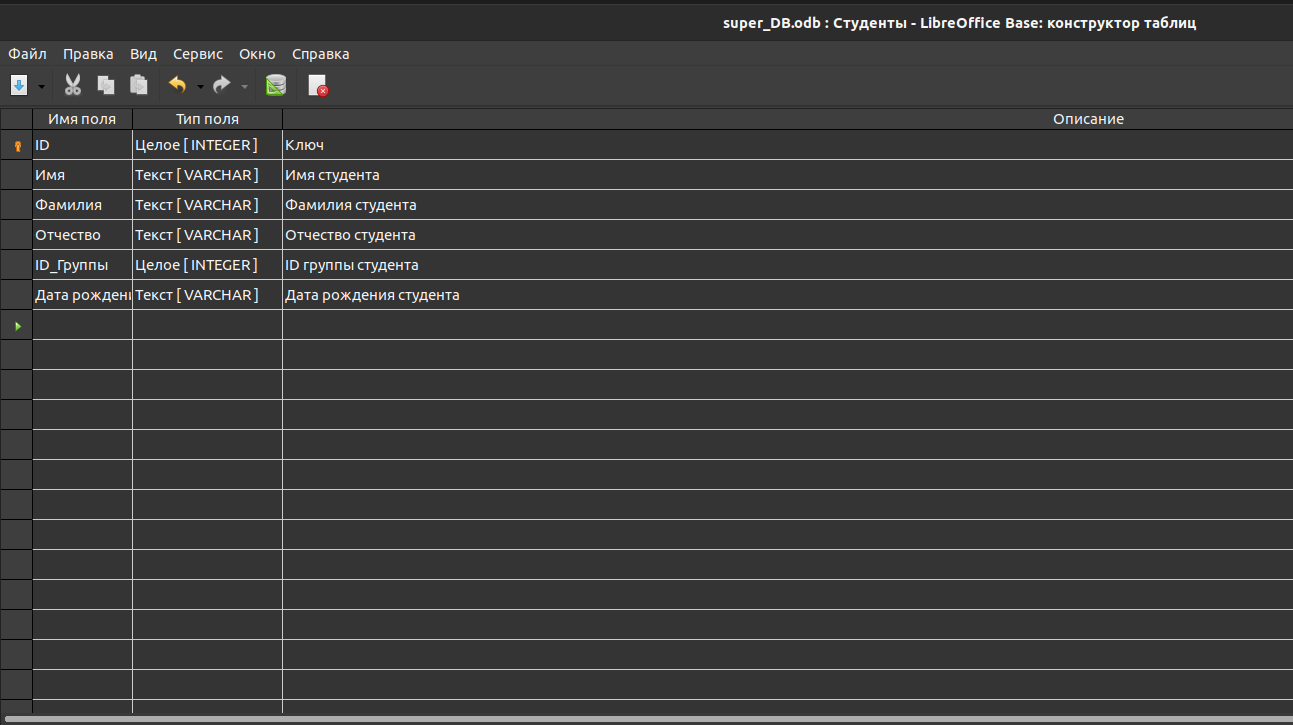
\includegraphics[width=\textwidth]{db3_construct.png}
  \caption{Создание таблицы}\label{ris:construct}}
\end{figure}

Каждая колонка таблицы имеет имя, которое задается в графе Имя поля. Хорошей практикой, особенно для таблиц с большим количеством колонок, является заполнение графы Описание. Тип поля заполняется путем выбора из вариантов, какого типа будет поле (текст, целые числа, дата).

Первая строка в таблице (ключ), является ключевым полем. Данные в ней будут появляться автоматически при добавлении каждой новой записи. Здесь это просто номер, который каждый раз увеличивается на единицу. Ключевое поле гарантирует, что в базе ни при каких обстоятельствах не будет содержаться двух одинаковых записей. Они обязательно будут отличаться друг от друга хотя бы ключом. Этого требует технология реляционных баз данных. Если ключевое поле не было создано, Дизайнер обратит на это внимание и предложит его создать.

\subsubsection{Наполнение таблиц}

Созданные таблицы отображаются во вкладке Таблицы главного меню. Если нажать на значек таблицы откроется окно ввода данных. Таблицы заполняются вручную или импортируются из заранее подготовленной электронной таблицы. Пример заполненой таблицы на рис.\ref{ris:tabins}

\begin{figure}[h]
\center{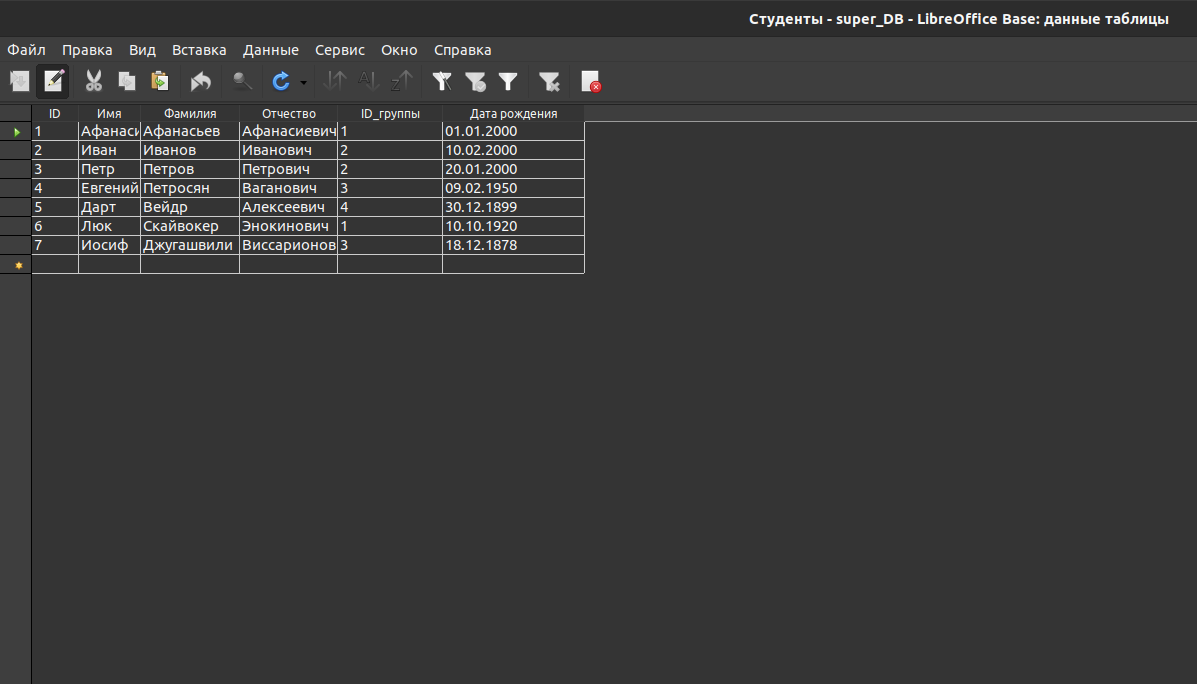
\includegraphics[width=\textwidth]{db_tabins.png}
  \caption{Таблица студенты}\label{ris:tabins}}
\end{figure}

\subsubsection{Создание запросов}

\textbf{Запрос (query)} --- это средство выбора необходимой информации из базы данных. Применяются два типа запросов: по образцу QBE и структурированный язык запросов SQL.

\textbf{QBE – Query by example} – средство для отыскания необходимой информации в базе данных. Он формируется не на специальном языке, а путем заполнения бланка запроса в окне Конструктора запросов.

\textbf{SQL --- Structured Query Language} --- это запросы, которые составляются (программистами) из последовательности SQL --- инструкций. Эти инструкции задают, что надо сделать с входным набором данных для генерации выходного набора.

Существует несколько типов запросов: на выборку, на обновление, на добавление, на удаление, перекрестный запрос, создание таблиц. Наиболее распространенным является запрос на выборку. Запросы на выборку используются для отбора нужной пользователю информации, содержащейся в таблицах. Они создаются только для связанных таблиц.

Так как для ипользования SQL потребуется дополнительные знания синтаксиса языка и понимание основ программирования, \textbf{можно использовать QBE}. Но стоит заметить что SQL имеет большую выразительную силу, и позволет быстрее описать желаемый результат. Далее в примерах будет использоватся SQL.

Для создания запросов необходимо перейти во кладку запросы и выбрать Создать запрос в режиме SQL. После того как запрос будет написан, необходимо нажать на значек выполнить запрос или нажать на клавишу F5. LibreOffice Base обработает запрос и вернет результат Рис. \ref{ris:selection}.

\begin{figure}[h]
\center{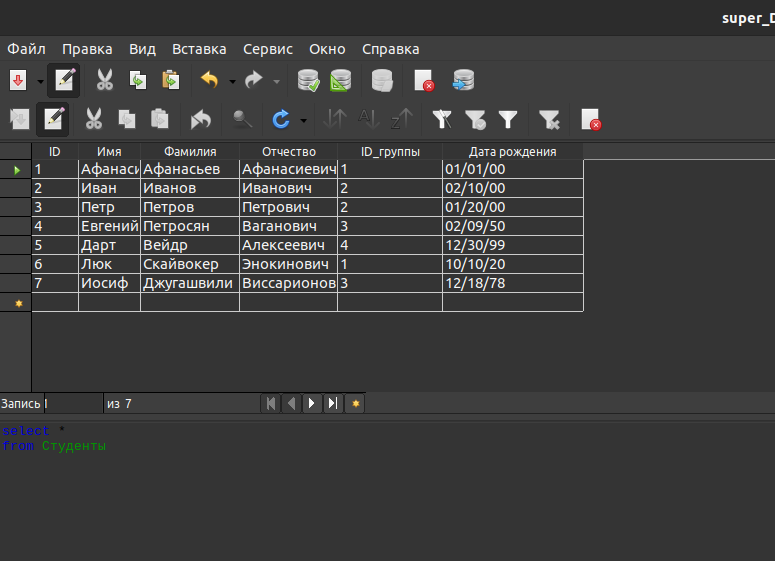
\includegraphics[width=\textwidth]{db_selection.png}
  \caption{Таблица студенты}\label{ris:selection}}
\end{figure}

\newpage
\begin{lstlisting}[label=select, caption=Базовая структура запроса]
SELECT
  [DISTINCT | DISTINCTROW | ALL]
  select_expression,...
FROM table_references
[WHERE where_definition]
[GROUP BY {unsigned_integer | col_name | formula}]
[HAVING where_definition]
[ORDER BY {unsigned_integer | col_name | formula} [ASC | DESC], ...]
\end{lstlisting}

\begin{lstlisting}[label=selection,caption=Выборка всех студентов]
  select *
  from Студенты
\end{lstlisting}

Ключевое слово \textbf{select} определяет список возвращаемых столбцов (как существующих, так и вычисляемых), их имена, ограничения на уникальность строк в возвращаемом наборе, ограничения на количество строк в возвращаемом наборе. Знак звезда (*) обозначает выборку всех столбцов результата запроса. Ключевое слово \textbf{from} задаёт табличное выражение, которое определяет базовый набор данных для применения операций, определяемых в других предложениях оператора т.е. указывает из каких таблиц делать выборку.

\newpage
\begin{lstlisting}[label=where, caption=Выборка студентов с датой рождения большей или равной условию]
  select *
  from Студенты
  where ДатаРождения >= {d '1950-02-01' }
\end{lstlisting}

\textbf{where} - оператор в SQL, указывающий, запрос должен действовать только на записи, удовлетворяющие определенным критериям. Критерии должны быть описаны в форме предикатов. Раздел WHERE — не обязательный раздел в SQL запросах. Он используется в качестве условия в SQL-запросе для ограничения записей обрабатываемых в выражениях SQL или возвращаемых запросом. В листинге \ref{where} оператор where задает условие выборки при котором должны отображатся только те студенты у которых день рождения больше или равно 1950.02.01. Для сравнения типа данных дата, в LibreOffice Base используются формат \{d 'ГГГГ-ММ-ДД'\}.

\begin{lstlisting}[label=order, caption=Запрос фамилий и дат рождения студентов отсортированных по дате рождения]
  select Фамилия, ДатаРождения
  from Студенты
  order by ДатаРождения desc
\end{lstlisting}

\textbf{order by} --- необязательный параметр оператора SELECT, который означает что запрос ,возвращают набор строк, отсортированных по значениям одного или более столбцов. Его можно применять как к числовым столбцам, так и к строковым. В последнем случае, сортировка будет происходить по алфавиту. Использование предложения ORDER BY является единственным способом отсортировать результирующий набор строк. Без этого предложения СУБД может вернуть строки в любом порядке. Если упорядочение необходимо, ORDER BY должен присутствовать в SELECT. Сортировка может производиться как по возрастанию, так и по убыванию значений. Параметр \textbf{ASC} (по умолчанию) устанавливает порядок сортировки по возрастанию, от меньших значений к большим. Параметр \textbf{DESC} устанавливает порядок сортировки по убыванию, от больших значений к меньшим.

\begin{lstlisting}[label=group, caption=Запрос количества телефонов у студентов]
select Фамилия, count( Телефон. НомерТелефона)
from Студенты, Телефон
where  Студенты.ID = Телефон.  ID студента
group by Фамилия
\end{lstlisting}

\textbf{group by} --- необязательный параметр операторa SELECT, для группировки строк по результатам агрегатных функций (MAX, SUM, AVG, COUNT, ...). Необходимо, чтобы в SELECT были заданы только требуемые в выходном потоке столбцы, перечисленные в GROUP BY и/или агрегированные значения. Распространённая ошибка — указание в SELECT столбца, пропущенного в GROUP BY.

\newpage
\subsection{Задание на лабораторную работу}

Для выполнения работы необходимо:
\begin{enumerate}
  \item Изучить теоретический материал
  \item Выбрать задание в соответствии с вариатом из таблицы \ref{tab:tasks}
  \item Создать базу данных
  \item Разработать таблицы с учетом нормализации (хотя бы 1НФ)
  \item Наполнить таблицы данными (минимум 10 строк)
  \item Создать 5 запросов:
    \begin{itemize}
      \item Выборка всех данных
      \item Выборка с условием
      \item Выборка с сортировкой
      \item Выборка с агрегатной функцией
      \item Выборка с условием на результат агрегатных функций
    \end{itemize}
  \item Оформить отчет по лабораторной работе
\end{enumerate}

\begin{table}[h]
      \caption{Варианты заданий}
      \begin{center}\label{tab:tasks}
        %\toprule
      \begin{tabular}{|c|c|}
        \hline
        Вариант & Описание задания \\
        \hline
        1 & База данных товаров в магазине\\
        2 & База данных авиарейсов\\
        3 & База дынных работников предприятия\\
        4 & База данных автомобилей\\
        5 & База данных преподавателей\\
        6 & База дынных городов\\
        7 & База данных стран\\
        8 & База данных компаний\\
        9 & База данных акций\\
        10 & База данных принцесс из диснея \\
        \hline
      \end{tabular}
    \end{center}
\end{table}


\newpage
\subsection{Содержание отчета}
\begin{enumerate}
  \item Титульный Лист
  \item Цель работы
  \item Краткие теоретические сведения по теме лабораторной работы
  \item Выполненное задание
  \item Краткий вывод о проделанной работе
\end{enumerate}

\subsection{Литература}



\end{document}
